\section{Results}\label{sec:results}

\subsection{The one-dimensional test (P1, P2)}\label{sec:beamres}
\paragraph{Uniform invariance.} Rotating every ply of the symmetric beam uniformly to
$20^\circ$ or $45^\circ$ lowers the linear frequency to $\nBUnifFTwenty$ and $\nBUnifFFortyFive$ of the
UD value ($\nBUDf$\,Hz). On the full FE model, the cubic SSM detuning coefficient is
unchanged to four digits (ratio $\nBUnif$), as Corollary~\ref{cor:beaminv} requires.
No uniform layup can therefore change $J$ at all.

\paragraph{Steering.} Table~\ref{tab:beam} and Fig.~\ref{fig:beam} report the optimized
symmetric beams. Every design has $\bm B\equiv\bm 0$, so the bending--extension
coupling plays no role. The optimizer does exactly what Proposition~\ref{prop:beam}
predicts: it turns the fibers off-axis in two zones centered, to within the knot spacing of the
angle field ($x/L=0.25$, $0.75$), on the inflection points ($x/L=0.224,0.776$), where $\varphi''^2$ vanishes, and keeps them axial where the beam
bends (Fig.~\ref{fig:beam}b). The SSM of the full FE beam confirms the condensed
evaluator's prediction for every design to within $\nBeamCondFE$ in $J/J_{\UD}$.
\begin{itemize}[itemsep=1pt]
\item \textbf{Tow-curvature limits.} At the $900^\circ$/m limit and $\omega_1\ge0.98\,
  \omega_{1,\UD}$, the detuning falls by $\nBNineHeldRed\%$. At $1800^\circ$/m it falls
  by $\nBEighteenHeldRed\%$, and with no tow limit by $\nBInfHeldRed\%$.
\item \textbf{Frequency allowance.} Relaxing the frequency to $0.90\,\omega_{1,\UD}$ gives
  $\nBNineNinetyRed\%$, $\nBEighteenNinetyRed\%$ and $\nBInfNinetyRed\%$ respectively.
\item \textbf{The coupling alternative.} The intuitive alternative is an unsymmetric
  laminate whose bending--extension coupling $\bm B(x)$ injects a softening quadratic
  force. We optimize it with its own, related objective (the RMS backbone drift over
  $a/h\le0.4$; two independently steered plies with two sine modes each, the same tow
  limit, and $\omega_1\ge0.90\,\omega_{1,\UD}$). It reduces that drift by only
  $\nBBred\%$, at $\nBBf\,\omega_{1,\UD}$. The comparison is therefore not like-for-like in
  objective, but the gap (a few percent against $\nBNineNinetyRed\%$ for symmetric steering at the same $900^\circ$/m limit and frequency floor) is far larger than the
  difference between the two objectives.
\end{itemize}
The lever on a clamped beam is therefore the spatial separation of curvature and
stretch, \emph{not} the bending--extension coupling. Its size is set by how narrow the
compliant zones can be (Corollary~\ref{cor:bang}). With no tow limit the two zones are each
$\approx0.05L$ wide at near-transverse fibers (total compliant length $\ell\approx0.1L$), and
\eqref{eq:bang} gives
$J/J_{\UD}\approx0.4$--$0.5$, against the computed $\nBInfHeld$. At $900^\circ$/m a
$90^\circ$ turn needs a third of the span, so the zones cannot both be narrow and
reach low modulus. This is why that limit binds.

\begin{table}[t]
\centering\footnotesize
\caption{Symmetric steered beam: detuning ratio $J/J_{\UD}$ from the condensed evaluator
(optimizer) and from the full FE + cubic SSM (confirmation), with the realized frequency
ratio.}\label{tab:beam}
\begin{tabular}{@{}lcccc@{}}
\toprule
tow limit & frequency floor & $J/J_{\UD}$ condensed & $J/J_{\UD}$ FE+SSM & $\omega_1/\omega_{1,\UD}$ (SSM)\\ \midrule
$900^\circ$/m & $0.98$ & $\nBNineHeldCond$ & $\nBNineHeld$ & $\nBNineHeldf$\\
$900^\circ$/m & $0.90$ & $\nBNineNinetyCond$ & $\nBNineNinety$ & $\nBNineNinetyf$\\
$1800^\circ$/m & $0.98$ & $\nBEighteenHeldCond$ & $\nBEighteenHeld$ & $\nBEighteenHeldf$\\
$1800^\circ$/m & $0.90$ & $\nBEighteenNinetyCond$ & $\nBEighteenNinety$ & $\nBEighteenNinetyf$\\
none & $0.98$ & $\nBInfHeldCond$ & $\nBInfHeld$ & $\nBInfHeldf$\\
none & $0.90$ & $\nBInfNinetyCond$ & $\nBInfNinety$ & $\nBInfNinetyf$\\
\bottomrule
\end{tabular}
\end{table}

\begin{figure}[t]
\centering
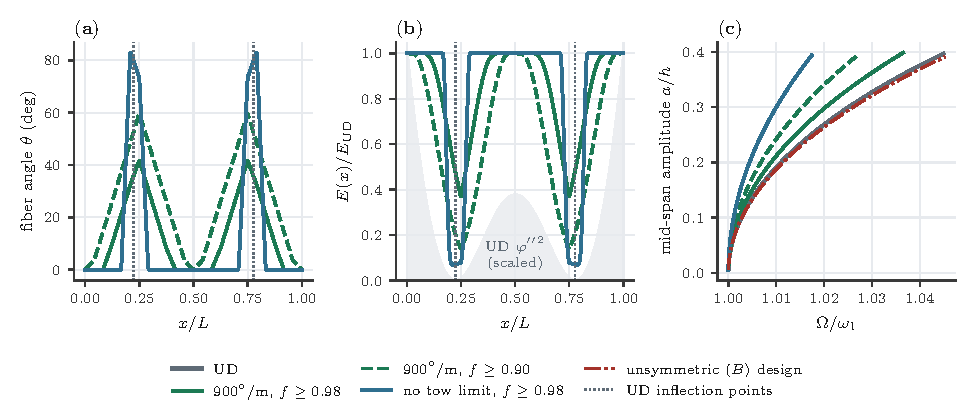
\includegraphics[width=\linewidth]{figs/fig_beam.pdf}
\caption{The one-dimensional test. \textbf{(a)}~Optimized mirror-symmetric fiber angle
of the symmetric ($\bm B=\bm0$) clamped beam for three designs: tow limit $900^\circ$/m
with the frequency held to $f\geq0.98$ or $f\geq0.90$ of the UD value, and no tow limit
with $f\geq0.98$. The UD beam ($\theta\equiv0$, $E=E_{\UD}$) appears in (c) only.
\textbf{(b)}~The axial modulus these fields produce, against the UD curvature weight
$\varphi''^2$ that sets $\omega_1^2$ (shaded). Fibers turn compliant where the beam does
not bend: the inflection points (dotted). \textbf{(c)}~Mid-span backbones from the full FE
beam and its cubic SSM; steering flattens the backbone markedly. (The optimized
unsymmetric, $\bm B$-coupled laminate was computed on a different beam model and objective,
so it is compared in the text, not plotted.)}
\label{fig:beam}
\end{figure}

\subsection{The achievable frequency--hardening set of the plate (P3)}\label{sec:levers}
Figure~\ref{fig:levers}a places every design class in the plane
$(\omega_1/\omega_{1,\UD},\,J/J_{\UD})$ at the same mass.

\paragraph{Uniform layups.} A uniform single angle traces a one-parameter curve. As
$\theta$ grows from $0^\circ$ the plate stiffens (up to $\nUfmax\,\omega_{1,\UD}$ at
$90^\circ$, fibers across the short span), and $J$ first falls to $\nUJmin$ at
$\theta=\nUthJmin^\circ$, where $\omega_1=\nUfatJmin\,\omega_{1,\UD}$, then rises. The
$\nSnum$ uniform symmetric stacks on a $15^\circ$ grid fill a region with a global
minimum of $\nSmin$ at $\nSfatmin\,\omega_{1,\UD}$. A grid envelope is not the strongest
uniform competitor: between grid points the continuous single angle already beats it
($\nUEleven$ vs.\ $\nGEleven$ at $1.1\,\omega_{1,\UD}$). We therefore also optimize the
four ply angles of $[\theta_4/\theta_3/\theta_2/\theta_1]_s$ \emph{continuously} at each
held frequency (SLSQP with the frequency equality, 22 starts from the best grid stacks,
the single-angle solution and random stacks; \texttt{stack\_continuous.py}). The best
uniform laminate reaches $J/J_{\UD}=\nCSEleven$, $\nCSTwelve$ and $\nCSThirteen$ at
$1.1$, $1.2$ and $1.3\,\omega_{1,\UD}$.

\paragraph{The UD floor.} Corollary~\ref{cor:udfloor} proves, and the enumeration confirms, that
the UD plate is the \emph{lowest-frequency} member of the whole
uniform family: the smallest stack frequency is $\nSfmin\,\omega_{1,\UD}$. At
exactly $\omega_1=\omega_{1,\UD}$ the continuous stack optimum is UD itself (all ply angles
$\to0$); the best grid stack within $\pm1\%$ of that frequency, at a slightly different
$\omega_1$, has $J/J_{\UD}=\nSheld$, a negligible difference. For a plate
mandated to the UD frequency, the uniform design space is therefore a single point.

\paragraph{Steered designs.} At exactly $\omega_{1,\UD}$, the steered single ply reaches
$J/J_{\UD}=\nFTen$, a $\nFTenRed\%$ reduction, with $R_{\min}=\SI{20}{mm}$ imposed (it is active but changes $J$ only in the fourth digit: without
it the optimum is $\nResAInf$, Sec.~\ref{sec:limits}). The steered designs lie well below the best uniform laminate at
\emph{every} frequency we test: $\nFEleven$, $\nFTwelve$ and $\nFThirteen$ at $1.1$,
$1.2$ and $1.3\,\omega_{1,\UD}$, against $\nCSEleven$, $\nCSTwelve$ and $\nCSThirteen$
for the best continuous stacks. Steering can also \emph{lower} the frequency below the uniform floor
($\nFNine$ at $0.9\,\omega_{1,\UD}$), which no uniform laminate can do. Steering the best
stack at $\omega_{1,\UD}$ gives $\nSFTen$, no better than the steered single ply. For
this plate and objective, the in-plane channel of Sec.~\ref{sec:channels} dominates the
through-thickness channel. Prediction P3 holds with a wide margin.

\begin{figure}[t]
\centering
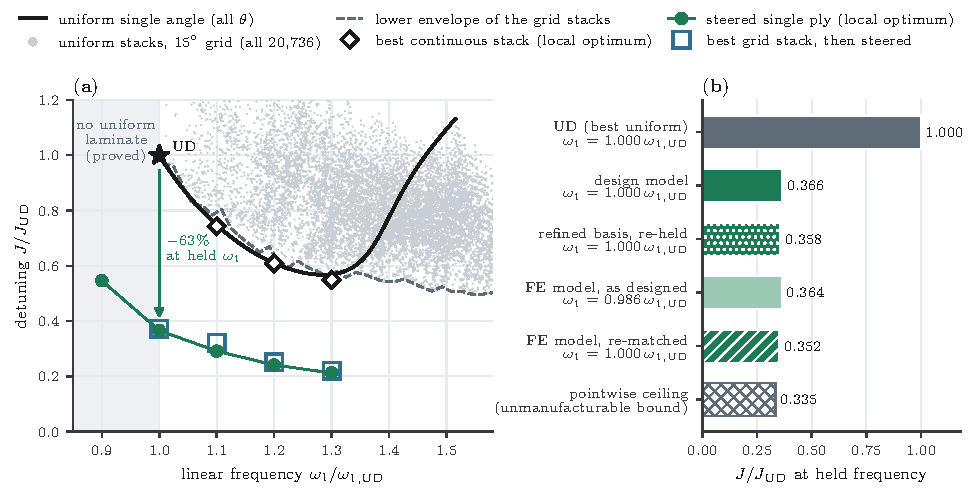
\includegraphics[width=\linewidth]{figs/fig_levers.pdf}
\caption{What each laminate freedom can reach, at fixed mass. \textbf{(a)}~Linear
frequency vs.\ frequency-normalized hardening. Black: uniform single angle. Gray dots:
$\nSnum$ uniform symmetric stacks on a $15^\circ$ grid (cloud clipped at $J/J_{\UD}=1.2$ and $\omega_1/\omega_{1,\UD}=1.58$),
with their lower envelope dashed; open diamonds: the best \emph{continuous} stack at each
held frequency, the strongest uniform competitor. Dotted vertical line:
$\omega_1=\omega_{1,\UD}$. Green: steered
single ply, optimized at five target frequencies with $R_{\min}=\SI{20}{mm}$. Blue
squares: the best $15^\circ$-grid stack at each target, then steered (where the two coincide, the green
dot sits inside the square; at $0.9\,\omega_{1,\UD}$ no uniform stack exists, so there is
no square). The UD plate (star) is the
lowest-frequency uniform laminate. \textbf{(b)}~At $\omega_1=\omega_{1,\UD}$: UD, which is
also the best uniform laminate there (Corollary~\ref{cor:udfloor}), the steered single ply, and
the unmanufacturable pointwise ceiling of Sec.~\ref{sec:limits}. The best stack at this
frequency is UD to within $\nGridStackDiff\%$ in $J$ ($[0/0/0/15]_s$), and steering it gives
$\nSFTen$, so it is not shown separately.}
\label{fig:levers}
\end{figure}

\subsection{The mechanism (P4)}\label{sec:mechanism}
Figure~\ref{fig:mechanism} tests the mechanism of Sec.~\ref{sec:theory} directly.
\begin{itemize}[itemsep=1pt]
\item \textbf{Where the energies live.} Both energies of the UD mode peak at the center.
  The bending energy is concentrated there, with the principal curvature along $y$, across
  the short span (panel a). The relaxed-stretch energy lies in a band along $x$ through
  the center, with its across-stretch direction along $x$ there and turning toward the
  corners (panel b).
\item \textbf{Sign of the trade-off.} At the held UD frequency the multiplier is negative,
  $\Lambda=\nLambda$ (dimensionless: $e_G$ and $e_K$ normalized by the UD $\gamma$ and
  $\omega_1^2$): minimizing the stretch energy alone would raise the frequency to
  $\nFreeFreq\,\omega_{1,\UD}$, so the constraint pushes the fibers \emph{across} the
  curvature. At the center the two preferences agree (fibers along $x$), and the pointwise design
  $\theta^\star$ keeps the UD direction there.
\item \textbf{Conflict.} Away from the center the across-stretch and across-curvature
  directions separate (panel c); their energy-weighted mean angle is $\nConflict^\circ$.
  This is where a single angle must compromise.
\item \textbf{Pointwise prediction.} The first-order design $\theta^\star(\bm x)$ of
  Proposition~\ref{prop:pointwise}, computed from the UD fields alone with no optimizer
  and no smoothness (panel d), already gives $J/J_{\UD}=\nStarJ$ when evaluated on the
  full model. Its frequency is $\nStarF\,\omega_{1,\UD}$, because the frozen-field model
  ignores the adaptation of the mode.
\item \textbf{Optimized field.} The optimized, curvature-limited field (panel e) shares the
  large-scale pattern of $\theta^\star$ (fibers turned off-axis toward the short edges) but
  departs from it in detail: the energy-weighted RMS angle difference is $\nStarDev^\circ$
  over the plate and $\nStarDevHigh^\circ$ where the energies are large, and at the energy
  peak the optimum is tilted to $\nOptAtPeak^\circ$. The frozen-field design ignores the
  adaptation of the mode and the smoothness and tow limit of a manufacturable field, both
  of which the optimizer must respect.
\end{itemize}

Panel f shows which terms move, normalized by UD:
\begin{itemize}[itemsep=1pt]
\item the raw (restrained) membrane cubic falls to $k_{nl}=\nDknl$;
\item the relaxation $2\bm g^{\!\top}\bm K_{\mathrm{in}}^{-1}\bm g$ changes to $\nDrelax$ of
  its UD value, a share of $k_{nl}$ rising from $\nRelaxUD\%$ to $\nRelaxOpt\%$;
\item the relaxed cubic falls to $\gamma=\nDgamma$;
\item the frequency is held ($\omega_1^2=\nDomsq$) and the mode's center value changes to
  $w_c=\nDmid$.
\end{itemize}
The hardening falls mainly through the direct term of \eqref{eq:gamma}: fibers across the
principal stretch store less membrane energy for the same stretch, so $k_{nl}$ falls to
$\nDknl$ of its UD value. The relaxation falls less (to $\nDrelax$), so its share of the
stretch energy rises and $\gamma$ falls further than $k_{nl}$ alone. Prediction P4 holds
partly: $\theta^\star$ alone captures most of the gain, though at $\nStarF\,\omega_{1,\UD}$, but the optimum departs from it by $\nStarDevHigh^\circ$ RMS even where the
energies are large.

\begin{figure}[t]
\centering
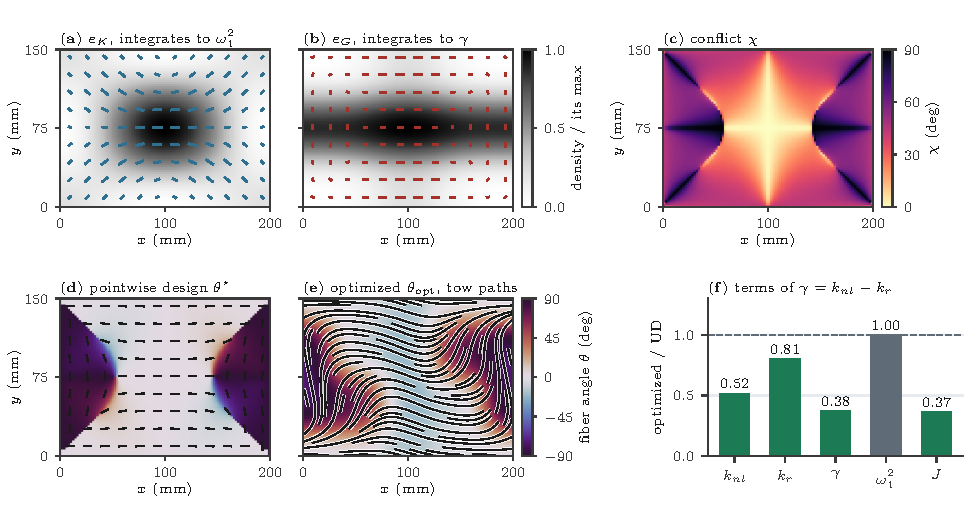
\includegraphics[width=\linewidth]{figs/fig_mechanism.pdf}
\caption{The mechanism. \textbf{(a)}~Bending-energy density $e_K$ of the UD fundamental
(it integrates to $\omega_1^2$), with the fiber direction that locally maximizes it
(principal curvature; green ticks, length $\propto$ anisotropic amplitude).
\textbf{(b)}~Relaxed-stretch density $e_G$ (integrates to $\gamma$), with the direction
that locally minimizes it (across the principal stretch; red ticks).
\textbf{(c)}~Conflict angle between the two preferred directions at the held frequency
($\Lambda<0$): across the stretch, $\varphi_G+90^\circ$, and across the curvature,
$\varphi_K+90^\circ$, i.e.\ the angle between the red ticks of (b) and the green ticks of
(a) rotated by $90^\circ$ (the green ticks show the curvature direction $\varphi_K$
itself, so at the center they are perpendicular to the red ticks and the conflict is
zero). The sharp ridges in (c) are lines where one of the two
principal directions is undefined (equal principal strains).
\textbf{(d)}~First-order pointwise design $\theta^\star$ from the UD fields alone
(Proposition~\ref{prop:pointwise}); black ticks: the same direction field; the cyclic color map is
lightest at $\theta=0^\circ$, so the pale regions are where $\theta^\star$ keeps the fibers along $x$.
\textbf{(e)}~Optimized curvature-limited field and its
tow paths. \textbf{(f)}~Optimized/UD ratios of the terms of \eqref{eq:gamma}, the raw cubic $k_{nl}$
and the relaxation $k_{r}=2\bm g^{\!\top}\bm K_{\mathrm{in}}^{-1}\bm g$, of their
difference $\gamma$, and of $\omega_1^2$ and $J$; dashed: parity with UD. All maps show the full
$\SI{200}{mm}\times\SI{150}{mm}$ plate; angles are measured from the $x$ axis.}
\label{fig:mechanism}
\end{figure}

\subsection{What bounds the lever (P5)}\label{sec:limits}
\paragraph{Anisotropy.} Along the family $\bm Q(s)=\bm Q_{\mathrm{iso}}+s(\bm Q-\bm
Q_{\mathrm{iso}})$, which keeps the isotropic invariants $U_1,U_4,U_5$ and scales $U_2,U_3$
by $s$, the held-frequency steered optimum falls monotonically with the anisotropy:
\begin{itemize}[itemsep=1pt]
\item $J/J_{\UD}=\nDoseA$ at $E_1/E_2=\nDoseRatioA$;
\item $\nDoseC$ at $\nDoseRatioC$;
\item $\nDoseE$ at $\nDoseRatioE$ (CFRP);
\item $\nDoseF$ at $\nDoseRatioF$ (Fig.~\ref{fig:limits}a).
\end{itemize}
The isotropic limit has no lever (Corollary~\ref{cor:iso}).

\paragraph{Tow curvature.} The held-frequency optimum degrades smoothly as the minimum
tow radius grows:
\begin{itemize}[itemsep=1pt]
\item $\nFrontThirty$ at $R_{\min}=\SI{30}{mm}$;
\item $\nFrontFifty$ at $\SI{50}{mm}$;
\item $\nFrontEighty$ at $\SI{80}{mm}$;
\item $\nFrontOneFifty$ at $\SI{150}{mm}$;
\item $\nFrontFourHundred$ at $\SI{400}{mm}$ (Fig.~\ref{fig:limits}b).
\end{itemize}
Below $R_{\min}\approx\SI{20}{mm}$ it saturates at $\nFrontTwenty$. Two checks show that
the saturation is physical rather than an artifact of the 50\,mm support grid.
\begin{itemize}[itemsep=1pt]
\item \textbf{Finer grid.} Refining the grid to 33\,mm and 25\,mm changes the optimum
  only to $\nResBTwenty$ and $\nResCTwenty$ at $R_{\min}=\SI{20}{mm}$, and to
  $\nResBInf$ and $\nResCInf$ with no tow limit.
\item \textbf{Pointwise ceiling.} Freeing $\theta$ at every quadrature point, with no
  smoothness and no tow limit (an unmanufacturable bound on single-ply steering), gives
  $\nCeil$.
\end{itemize}
The plate's strain fields vary on a length scale of a few centimeters. Once tows can
turn on that scale, further manufacturing freedom buys little. Prediction P5 holds:
the lever is set by the material anisotropy and by the ratio of the tow radius to the
length scale of the mode's strain fields.

\begin{figure}[t]
\centering
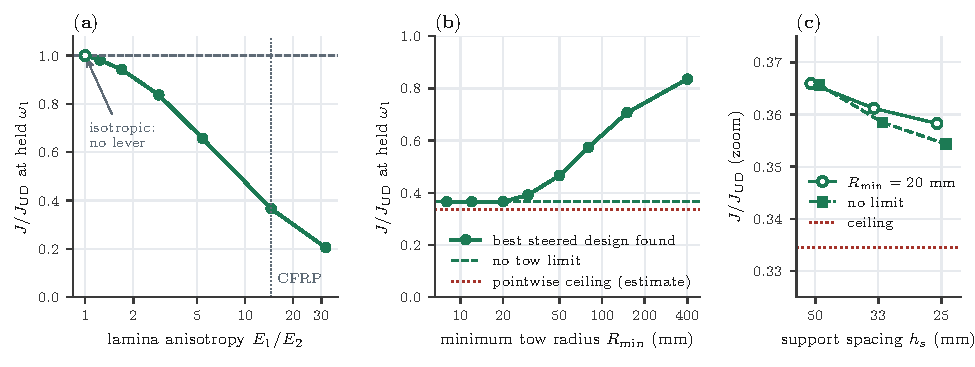
\includegraphics[width=\linewidth]{figs/fig_limits.pdf}
\caption{What bounds the lever, at held frequency. \textbf{(a)}~Steered optimum vs.\
lamina anisotropy along a family that scales only the anisotropic invariants
($E_1/E_2=1$ is isotropic, where $J/J_{\UD}=1$ exactly by Corollary~\ref{cor:iso}, so that point is
not computed; dashed: parity with UD; dotted: CFRP). \textbf{(b)}~Manufacturability front: optimum vs.\ minimum tow
radius on the 50\,mm support grid; dashed: the same grid with no tow limit; dotted: the
pointwise (unmanufacturable) ceiling. \textbf{(c)}~Support-grid refinement (zoomed
ordinate; the three support spacings are plotted as equally spaced categories, with the two
series offset slightly for visibility): at $R_{\min}=\SI{20}{mm}$ (open) and with no tow limit (filled) the optimum
moves by less than $0.02$ and approaches the ceiling, so the saturation in (b) is physical,
not a parametrization artifact.}
\label{fig:limits}
\end{figure}

\subsection{Independent confirmation on the full model}\label{sec:confirm}
The design was produced on the condensed, adapted-mode evaluator. We confirm it on the
full multi-mode plate: 36 transverse and 72 in-plane modes, in-plane inertia retained,
an independent Gauss-quadrature assembly, and amplitudes measured as the true mid-plate
deflection (Table~\ref{tab:confirm}).
\begin{itemize}[itemsep=1pt]
\item \textbf{Full SSM.} The full cubic SSM gives detuning coefficients $\beta$ within
  $\nSSMvsEval\%$ of the evaluator for both designs. The detuning ratio is $\nCratioSSM$, a
  $\nCredSSM\%$ reduction.
\item \textbf{EPMC.} Full-order EPMC continuation ($H=\nEPMCH$ harmonics) gives a ratio of $\nCratioEPMC$.
\item \textbf{Frequency.} The steered design's full-model frequency is $\nCOptf$\,Hz
  against $\nCUDf$\,Hz for UD. The difference is the Ritz upper-bound convergence of the
  transverse basis for the steered field (Table~\ref{tab:conv}: the steered frequency
  falls by $\nConvFreqDrop\%$ from $m,n\le8$ to $m,n\le16$ while the UD frequency is unchanged), not a
  design change.
\item \textbf{Discretization.} An independent finite-element model (ACM Kirchhoff
  bending with Q4 membrane elements, Appendix~\ref{app:fe}) evaluated on the optimized
  field gives a detuning ratio of $\nFEratio$. Across the three discretizations the
  steered design's frequency lies within $\pm\nHeldTol\%$ of the UD value, which is the
  accuracy to which ``held frequency'' is meaningful here.
\end{itemize}

\begin{table}[t]
\centering\footnotesize
\caption{Confirmation of the held-frequency design. $\beta$: small-amplitude coefficient
of $\Om/\omega_1-1=\beta(a/h)^2$ at the plate center.}\label{tab:confirm}
\begin{tabular}{@{}lcccc@{}}
\toprule
model & $f_1$ UD (Hz) & $f_1$ steered (Hz) & $\beta$ UD & $\beta$ steered\\ \midrule
design evaluator (64+72 modes, condensed) & $\nUDf$ & $\nUDf$ & $\nEvBetaUD$ & $\nEvBetaOpt$\\
full plate, cubic SSM (36+72 modes) & $\nCUDf$ & $\nCOptf$ & $\nCUDbetaSSM$ & $\nCOptbetaSSM$\\
full plate, EPMC ($H=\nEPMCH$) & --- & --- & $\nCUDbetaEPMC$ & $\nCOptbetaEPMC$\\
independent FE (ACM + Q4, $\nFEmesh$, App.~\ref{app:fe}) & $\nFEUDf$ & $\nFEOptf$ & $\nFEUDbeta$ & $\nFEOptbeta$\\
\bottomrule
\end{tabular}
\end{table}

\subsection{Consequence: a wider jump-free range}\label{sec:jumpres}
Proposition~\ref{prop:cusp} predicts that the held-frequency reduction widens the
jump-free amplitude by $(J_{\mathrm{steered}}/J_{\UD})^{-1/2}=\nCacTheory$. We compute
$a_c$ numerically as the drive at which the full-order damped SSM forced response
($\zeta=2\%$, center point load) first becomes multivalued. It rises from $a_c/h=\nCUDac$
to $\nCOptac$, a factor $\nCacRatio$ in amplitude and $\nCFratio$ in drive. This agrees
with the predicted ratio, and the absolute thresholds agree too: \eqref{eq:ac} with the
full-model $\beta$ gives $\nCacFormUD$ and $\nCacFormOpt$.

Direct time integration then shows the jump itself (Fig.~\ref{fig:confirm}b,c). We drive
both panels with the same point load, set between their two thresholds, and sweep the
frequency up and down. The UD panel is hysteretic: the up and down sweeps differ by up
to $\nCUDgap\,h$ across the fold. The steered panel, at the same frequency and mass, is
single-valued: its sweeps coincide to $\nCOptgap\,h$ and follow the SSM forced response. A finer
sweep ($\nFineSteps$ steps over $\Om/\omega_1\in[1.00,1.08]$; \texttt{confirm\_\allowbreak fine\_\allowbreak sweep.py})
confirms both: the UD up and down sweeps differ at $\nFineHyst$ consecutive steps across the
fold (by up to $\nFineGap\,h$), the steered sweeps at none.
\begin{figure}[t]
\centering
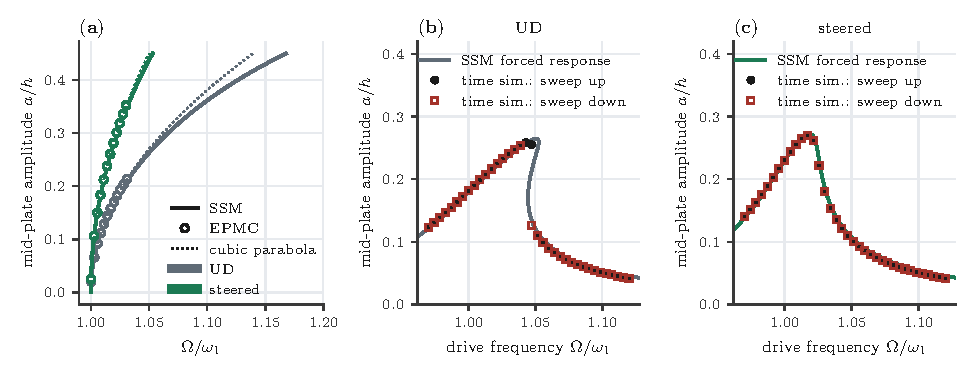
\includegraphics[width=\linewidth]{figs/fig_confirm.pdf}
\caption{Confirmation and consequence. \textbf{(a)}~Mid-plate backbones of the full
multi-mode plate: cubic SSM (lines) and full-order EPMC (markers), UD (gray) and the
held-frequency steered design (green). Dotted: the cubic parabola
$1+\beta(a/h)^2$ with the full-model SSM $\beta$ (within $\nSSMvsEval\%$ of the condensed evaluator's).
\textbf{(b,c)}~Time-integrated harmonic sweeps (up: black dots; down: red squares; 300
forcing periods per step, and a point is kept only once its amplitude is steady to $0.4\%$,
which excludes one UD point at the fold) at one
drive between the two jump thresholds, over the damped SSM forced response. The UD panel
folds and jumps. The steered panel, at the same linear frequency and mass, stays
single-valued.}
\label{fig:confirm}
\end{figure}
